\documentclass[14pt]{beamer}

% Presento style file
\usepackage{config/presento}
\usepackage{comment}
\usepackage{algorithm}
\usepackage[noend]{algpseudocode}

\renewcommand{\thealgorithm}{}

% custom command and packages
% custom packages
\usepackage{textpos}
\setlength{\TPHorizModule}{1cm}
\setlength{\TPVertModule}{1cm}

\newcommand\crule[1][black]{\textcolor{#1}{\rule{2cm}{2cm}}}



% Information
\title{deep RL for flexible decision-making}
\subtitle{}
\author{fede carnevale}
\institute{zador lab}
\date{neuro in-house \\ \today}

\begin{document}

% Title page
\begin{frame}[plain]
\maketitle
\end{frame}

%%%%%%%%%%%%%%%%%%%%%%%%%%%%%%%%%%%%%%%%%%%%%%%%%%%%%%
\begin{frame}{Motivation}

\largetext{
How do animals learn flexible behaviors that combine:
\begin{itemize}[label=$\bullet$]
  \item external stimuli
  \item context, rules
  \item prior knowledge
  \item reward contingencies
  \item ...
\end{itemize}
}

\end{frame}
%%%%%%%%%%%%%%%%%%%%%%%%%%%%%%%%%%%%%%%%%%%%%%%%%%%%%%

%%%%%%%%%%%%%%%%%%%%%%%%%%%%%%%%%%%%%%%%%%%%%%%%%%%%%%
\begin{frame}{RL mathematical framework}


  \begin{figure}[htb]
    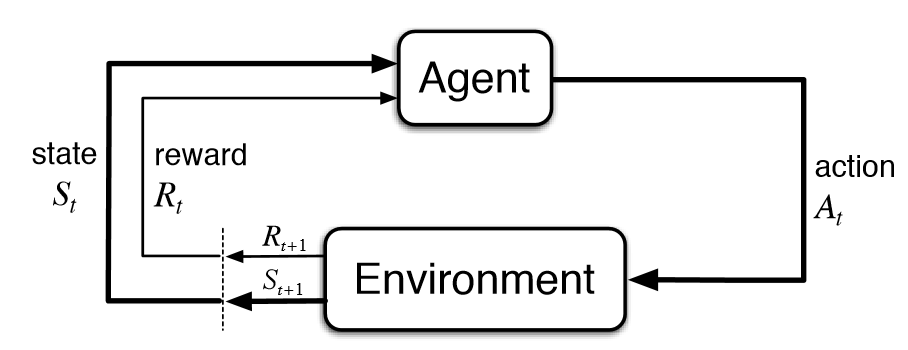
\includegraphics[width=0.8\textwidth]{images/rl}
  \end{figure}


  \begin{fullpageitemize}
  \item 
      \largetext{\color{colorblue}{Policy:}} $\pi \left( a \vert s \right) = \mathbb{P} \left( A_t = a \vert S_t = s \right) $
  \item 
      \largetext{\color{colorblue}{Value:}} $ V_{\pi}\left( s \right) = \mathbb{E} \lbrack R_{t+1} + \gamma R_{t+2} + ... \vert S_t = s\rbrack $
  \end{fullpageitemize}

\end{frame}
%%%%%%%%%%%%%%%%%%%%%%%%%%%%%%%%%%%%%%%%%%%%%%%%%%%%%%

%%%%%%%%%%%%%%%%%%%%%%%%%%%%%%%%%%%%%%%%%%%%%%%%%%%%%%
\begin{frame}{RL advances in the last years}

  \begin{figure}[htb]
  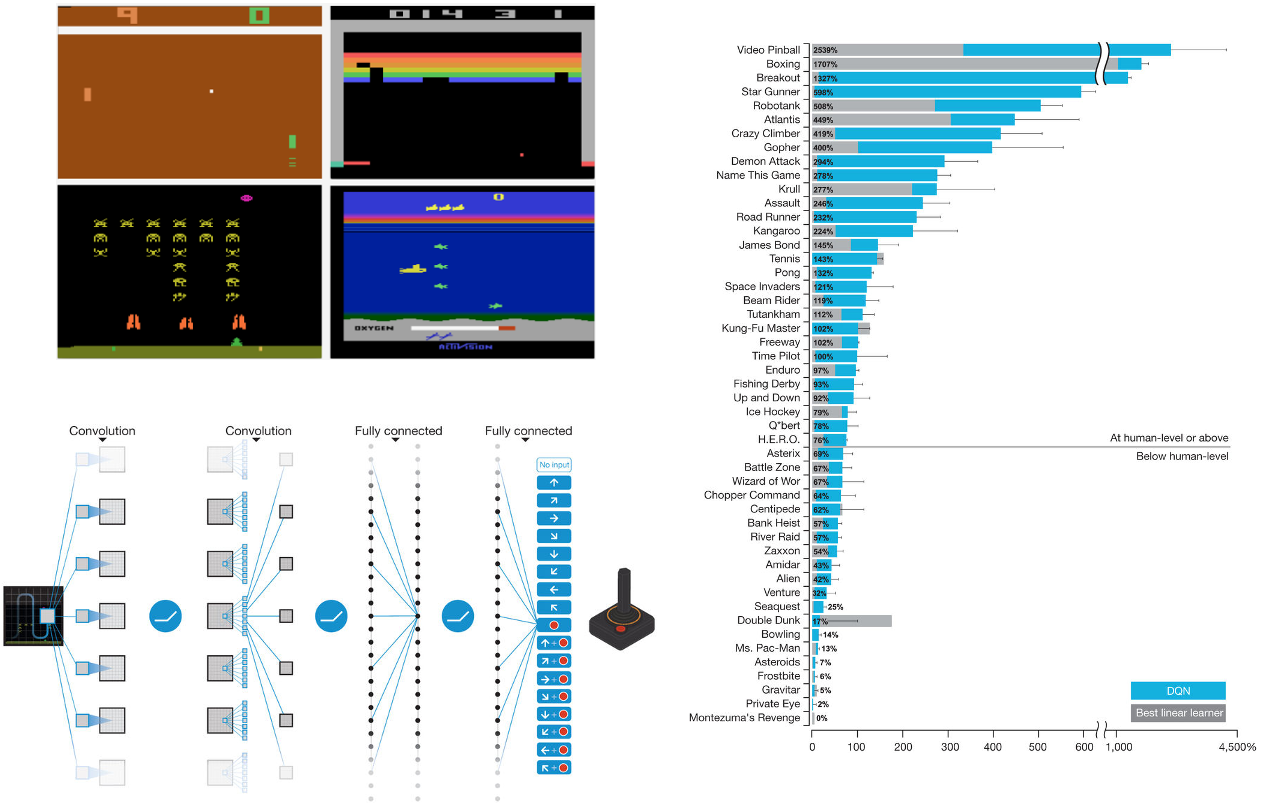
\includegraphics[width=0.9\textwidth]{images/dqn}
  \end{figure}

\setnote{Mnih et al, 2014}
\end{frame}
%%%%%%%%%%%%%%%%%%%%%%%%%%%%%%%%%%%%%%%%%%%%%%%%%%%%%%

%%%%%%%%%%%%%%%%%%%%%%%%%%%%%%%%%%%%%%%%%%%%%%%%%%%%%%
\begin{frame}{However,}

 \begin{itemize}
  \item - \largetext{data inefficiency}
  \item
  \item - \largetext{lack of flexibility}
 \end{itemize}

\vspace{0.75cm}
\color{colorblue}\largetext{Animals, in contrast, are capable of learning flexible behaviors much more efficiently}

\end{frame}
%%%%%%%%%%%%%%%%%%%%%%%%%%%%%%%%%%%%%%%%%%%%%%%%%%%%%%

%%%%%%%%%%%%%%%%%%%%%%%%%%%%%%%%%%%%%%%%%%%%%%%%%%%%%%
\begin{frame}{Aki's task}
  \begin{figure}[htb]
    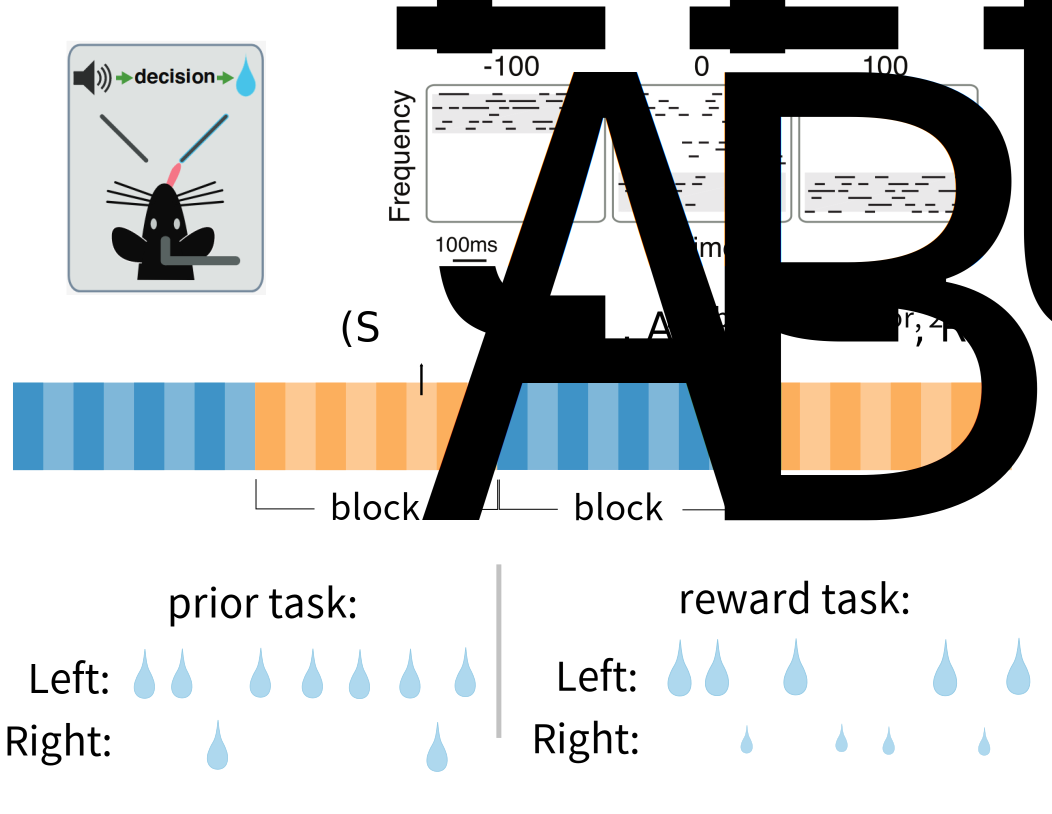
\includegraphics[width=\textwidth]{images/akitask}
  \end{figure}
\setnote{Marbach and Zador, 2016}
\end{frame}
%%%%%%%%%%%%%%%%%%%%%%%%%%%%%%%%%%%%%%%%%%%%%%%%%%%%%%

%%%%%%%%%%%%%%%%%%%%%%%%%%%%%%%%%%%%%%%%%%%%%%%%%%%%%%
\begin{frame}{An RL agent for aki's task}
  
% a feed forward nn could never solve the task, because it has no memory
% we want the model to respond differently depending on the block/context
% but the block has to be infered (there's no cue)
% the only way to infer is by using the sequence of s,a,r
% for sequential data, recurrent nn are used. 
\begin{figure}[htb]
  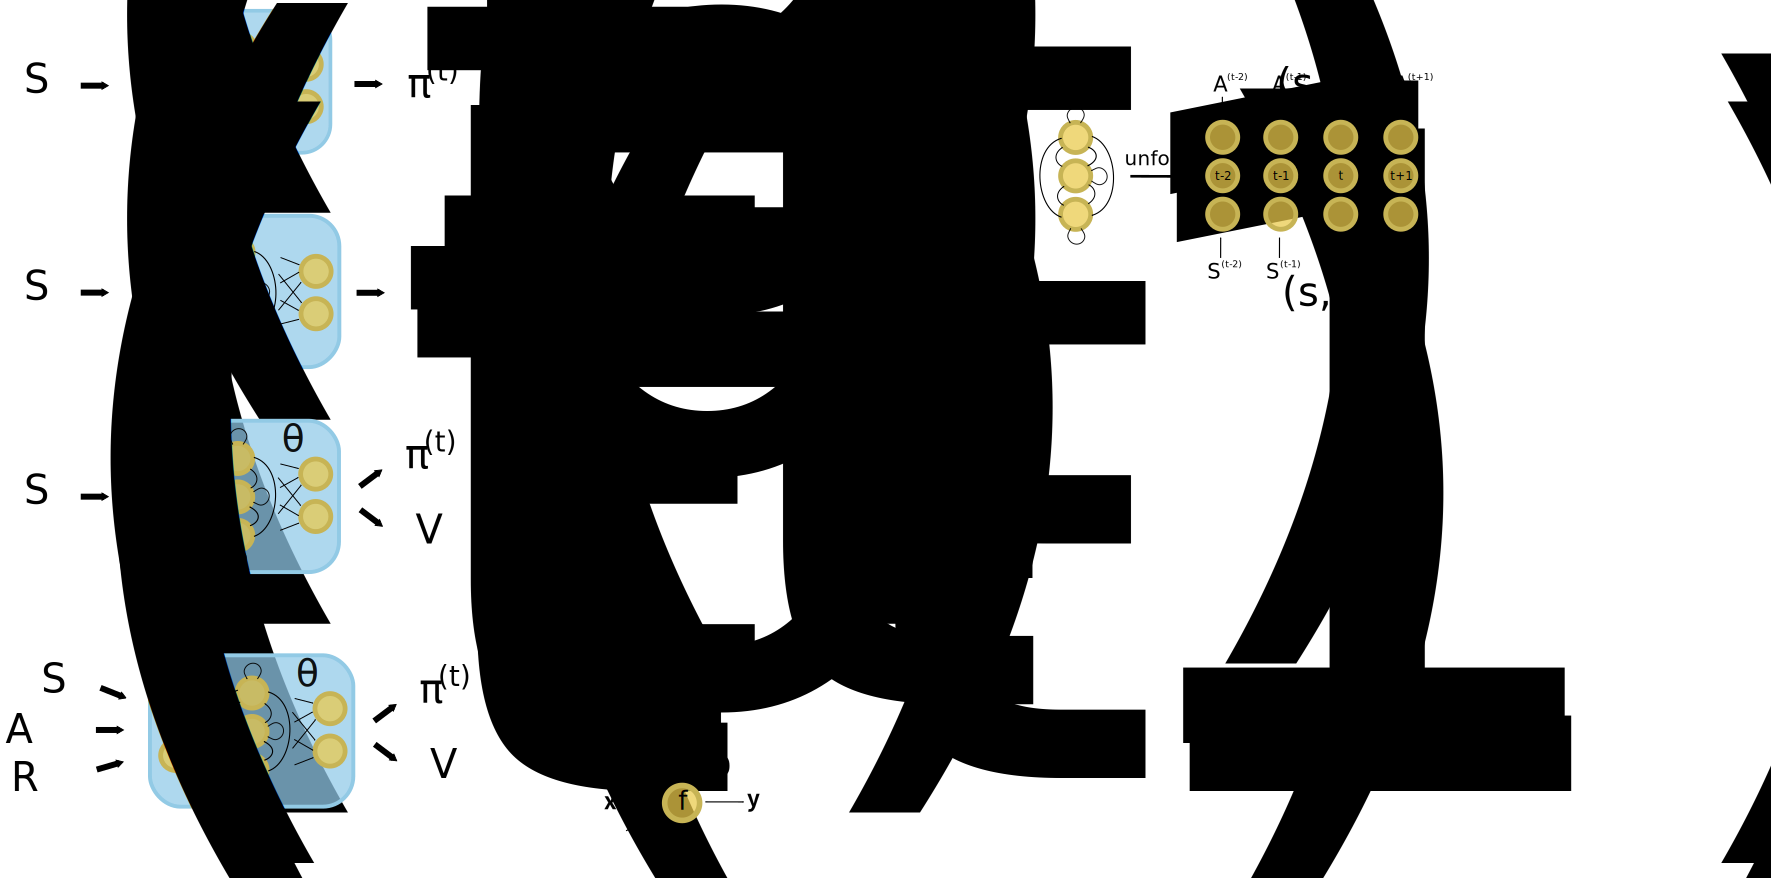
\includegraphics[width=0.9\textwidth]{images/ffnn}
\end{figure}

Find $\theta$ that maximizes $J(\theta) = \mathbb{E}_{\pi_{\theta}} \lbrack R \rbrack $

\vspace{0.2cm}

\begin{columns}

\begin{column}{0.1\textwidth}
\end{column}

\begin{column}{0.4\textwidth}
  \begin{figure}[htb]
    \includegraphics[width=\textwidth]{images/neuron}
  \end{figure}
\end{column}

\begin{column}{0.4\textwidth}
  \begin{align*}
    \mathbf{y} &= f \left(\mathbf{W} \mathbf{x} + \mathbf{b} \right)
  \end{align*}
\end{column}

\begin{column}{0.1\textwidth}
\end{column}

\end{columns}


\end{frame}
%%%%%%%%%%%%%%%%%%%%%%%%%%%%%%%%%%%%%%%%%%%%%%%%%%%%%%

%%%%%%%%%%%%%%%%%%%%%%%%%%%%%%%%%%%%%%%%%%%%%%%%%%%%%%
\begin{frame}{Recurrent Neural Networks}

\begin{figure}[htb]
  \includegraphics[width=0.9\textwidth]{images/rnn}
\end{figure}
\begin{align*}
  \mathbf{x}^{(t)} &= \mathbf{W} \mathbf{h}^{(t-1)} + \mathbf{U}  \mathbf{s}^{(t)} + \mathbf{b} \\
  \mathbf{h}^{(t)} &= \text{ tanh} \left( \mathbf{x}^{(t)} \right) \\
  \mathbf{o}^{(t)} &= \mathbf{V}  \mathbf{h}^{(t)} + \mathbf{c} 
\end{align*}

\color{colorblue}Recurrent connections allow previous inputs to persist (memory) and affect the output.

\end{frame}
%%%%%%%%%%%%%%%%%%%%%%%%%%%%%%%%%%%%%%%%%%%%%%%%%%%%%%

%%%%%%%%%%%%%%%%%%%%%%%%%%%%%%%%%%%%%%%%%%%%%%%%%%%%%%
\begin{frame}{Recurrent Neural Networks}

\begin{figure}[htb]
  \includegraphics[width=0.9\textwidth]{images/unfold}
\end{figure}

\begin{figure}[htb]
  \includegraphics[width=0.9\textwidth]{images/blocks}
\end{figure}

\end{frame}
%%%%%%%%%%%%%%%%%%%%%%%%%%%%%%%%%%%%%%%%%%%%%%%%%%%%%%

%%%%%%%%%%%%%%%%%%%%%%%%%%%%%%%%%%%%%%%%%%%%%%%%%%%%%%
\begin{frame}{Training procedure}

\begin{figure}[htb]
  \includegraphics[height=2.5cm]{images/rnn2}
\end{figure}

Find $\theta$ that maximizes $J(\theta) = \mathbb{E}_{\pi_{\theta}} \lbrack R \rbrack $

\begin{align*}
  \nabla_\theta \: J \left( \theta \right) = \mathbb{E}_{\pi_{\theta}} \lbrack \nabla_{\theta} log \: \pi_{\theta} \left( s,a \right) V^{\pi_{\theta}} \left( s \right) \rbrack \\
  \\
  \theta \leftarrow \theta + \alpha \nabla_{\theta} log \: \pi_{\theta} \left( s,a \right) V^{\pi_{\theta}} \left( s \right)
\end{align*}
\end{frame}
%%%%%%%%%%%%%%%%%%%%%%%%%%%%%%%%%%%%%%%%%%%%%%%%%%%%%%

%%%%%%%%%%%%%%%%%%%%%%%%%%%%%%%%%%%%%%%%%%%%%%%%%%%%%%
\begin{frame}{Training procedure}

\begin{figure}[htb]
  \includegraphics[height=2.5cm]{images/rnn2}
\end{figure}
%\begin{align*}
%  A_t  \: \textasciitilde \: \pi_\theta \left(s,a)\right) &= \mathbb{P} \left( a \vert s,\theta \right) \\
%  & \propto softmax(o^{(t)})
%\end{align*}

\smalltext{
\begin{algorithm}[H]
\caption{Reinforce}
\begin{algorithmic}
\State \smalltext{Initialize $\theta$ arbitrarily}
\State \smalltext{\textbf{for} each block $\left([s_1,a_1,r_1],...,[s_T,a_T,r_T] \right)$ \textbf{do}}
\State \smalltext{$\;$$\;$ \textbf{for} $t=1$ to $T$ \textbf{do}}
\State \smalltext{$\;\;\;\; \delta_v(s_t) = r_t + \gamma V(s_t) - V(s_{t-1})$}
\State \smalltext{$\;\;\;\; \theta \gets \theta + \alpha \nabla_\theta log \, \pi_\theta (s_t,a_t) \delta_v(s_t)$}
\State \smalltext{$\;\;$ \textbf{end for}}
\State \smalltext{\textbf{end for}}
\State \smalltext{\textbf{return} $\theta$}
\end{algorithmic}
\end{algorithm}
}
\end{frame}
%%%%%%%%%%%%%%%%%%%%%%%%%%%%%%%%%%%%%%%%%%%%%%%%%%%%%%

%%%%%%%%%%%%%%%%%%%%%%%%%%%%%%%%%%%%%%%%%%%%%%%%%%%%%%
\begin{frame}{Training procedure}

\begin{figure}[htb]
  \includegraphics[height=2.5cm]{images/rnn3}
\end{figure}

\end{frame}
%%%%%%%%%%%%%%%%%%%%%%%%%%%%%%%%%%%%%%%%%%%%%%%%%%%%%%

%%%%%%%%%%%%%%%%%%%%%%%%%%%%%%%%%%%%%%%%%%%%%%%%%%%%%%
\begin{frame}{The agent solves both tasks}

\begin{columns}

\begin{column}{0.5\textwidth}
  \begin{figure}[htb]
    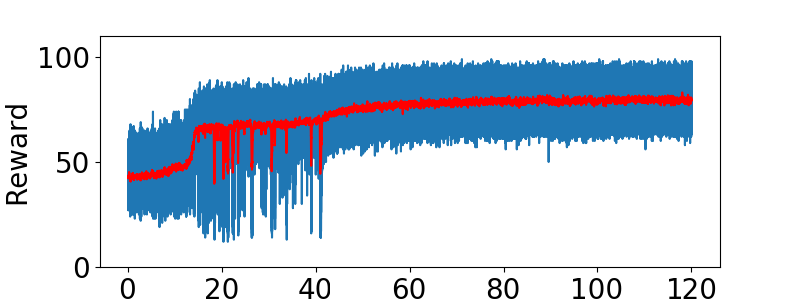
\includegraphics[width=\textwidth]{images/ptask/total_rew}
  \end{figure}
  \vspace{-0.5cm}
  \begin{figure}[htb]
    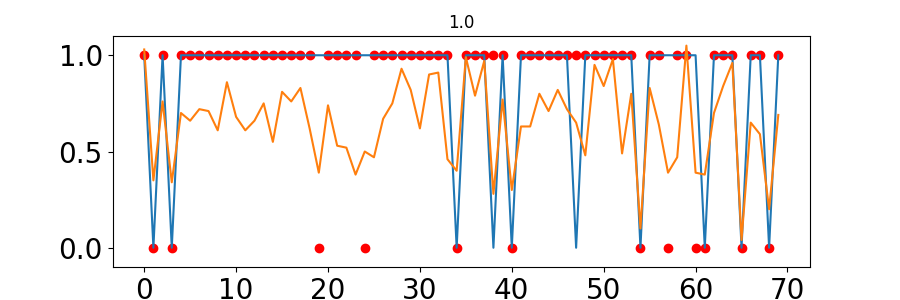
\includegraphics[width=\textwidth]{images/ptask/episode4}
  \end{figure}
  \vspace{-1cm}
  \begin{figure}[htb]
    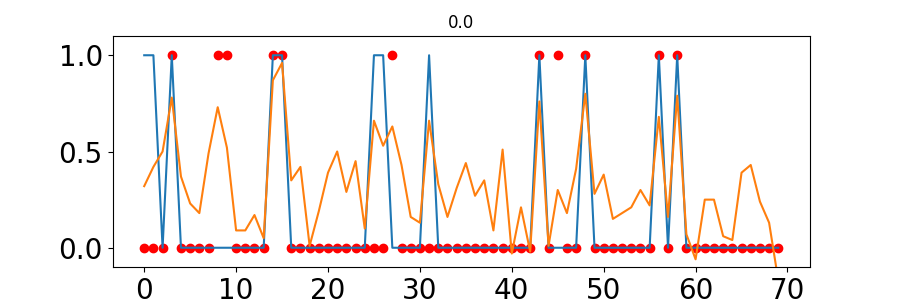
\includegraphics[width=\textwidth]{images/ptask/episode2}
  \end{figure}
\end{column}

\begin{column}{0.5\textwidth}
  \begin{figure}[htb]
    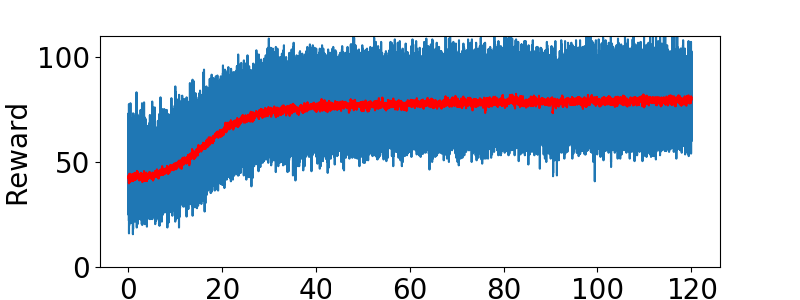
\includegraphics[width=\textwidth]{images/rtask/total_rew}
  \end{figure}
  \vspace{-0.5cm}
  \begin{figure}[htb]
    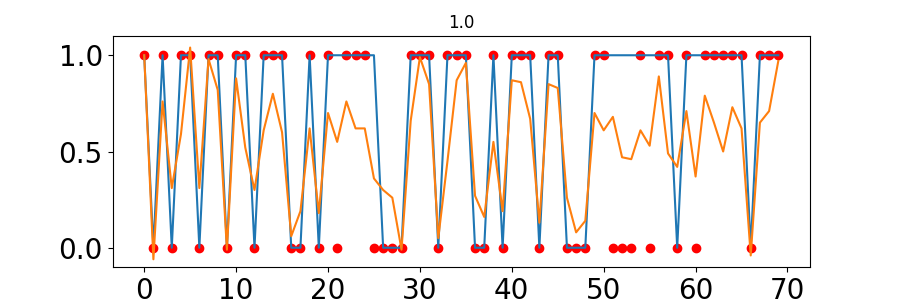
\includegraphics[width=\textwidth]{images/rtask/episode4}
  \end{figure}
  \vspace{-1cm}
  \begin{figure}[htb]
    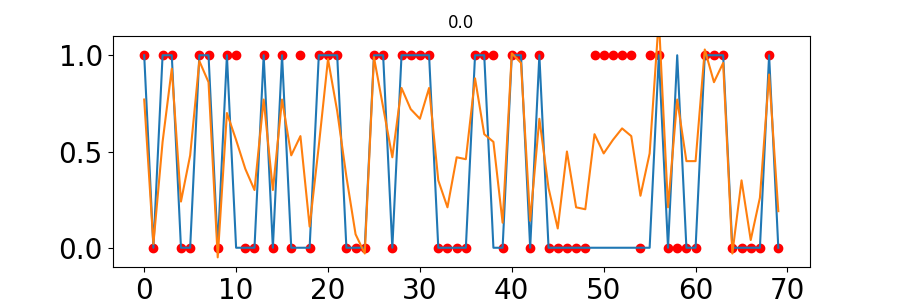
\includegraphics[width=\textwidth]{images/rtask/episode0}
  \end{figure}
\end{column}

\end{columns}


\end{frame}
%%%%%%%%%%%%%%%%%%%%%%%%%%%%%%%%%%%%%%%%%%%%%%%%%%%%%%


%%%%%%%%%%%%%%%%%%%%%%%%%%%%%%%%%%%%%%%%%%%%%%%%%%%%%%
\begin{frame}{Asym prior/reward biases choice}

  \begin{figure}[htb]
  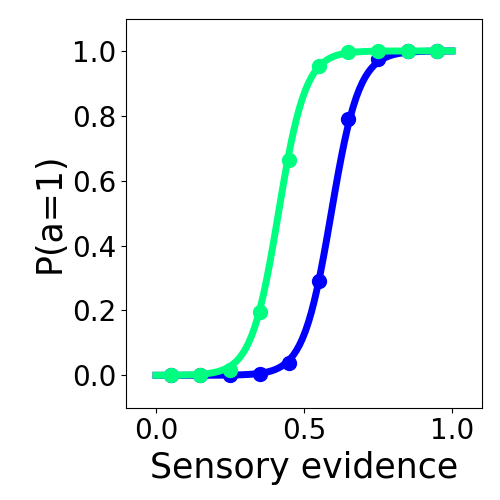
\includegraphics[width=0.7\textwidth]{images/ptask/avg_psycho}
  \end{figure}

\end{frame}
%%%%%%%%%%%%%%%%%%%%%%%%%%%%%%%%%%%%%%%%%%%%%%%%%%%%%%


%%%%%%%%%%%%%%%%%%%%%%%%%%%%%%%%%%%%%%%%%%%%%%%%%%%%%%
\begin{frame}{Bias develops within block}

\begin{columns}
\begin{column}{0.5\textwidth}

  \begin{figure}
  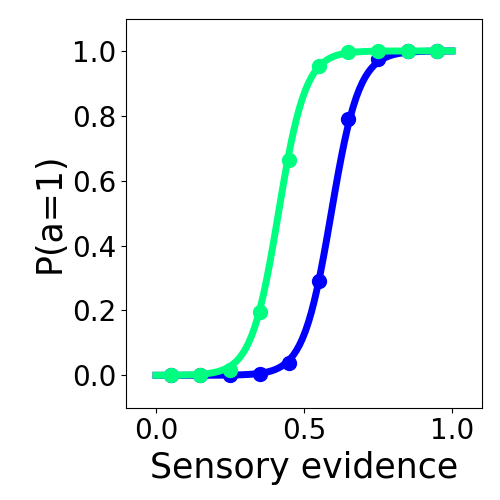
\includegraphics[width=\textwidth]{images/ptask/avg_psycho}
  \end{figure}

\end{column}
\begin{column}{0.5\textwidth}

  \begin{figure}
  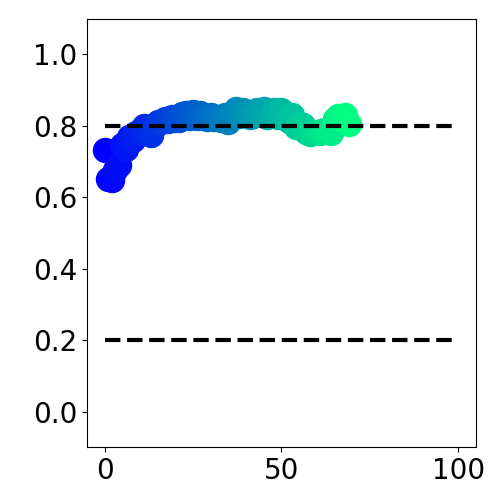
\includegraphics[width=0.7\textwidth]{images/ptask/time_bias1}
  \end{figure}
  \vspace{-2cm}
  \begin{figure}
    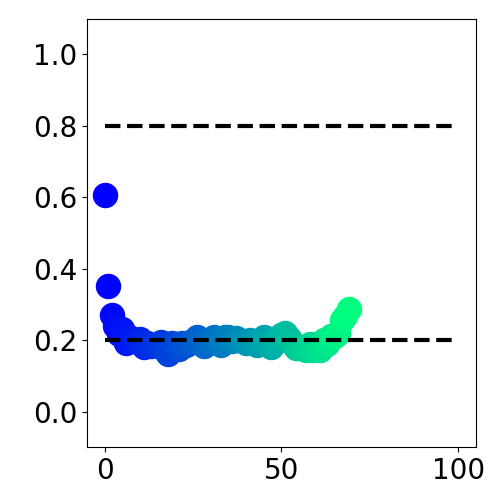
\includegraphics[width=0.7\textwidth]{images/ptask/time_bias0}
  \end{figure}

\end{column}
\end{columns}

\end{frame}
%%%%%%%%%%%%%%%%%%%%%%%%%%%%%%%%%%%%%%%%%%%%%%%%%%%%%%


%%%%%%%%%%%%%%%%%%%%%%%%%%%%%%%%%%%%%%%%%%%%%%%%%%%%%%
\begin{frame}{The agent can generalize to new priors/rewards}

  \begin{figure}[htb]
  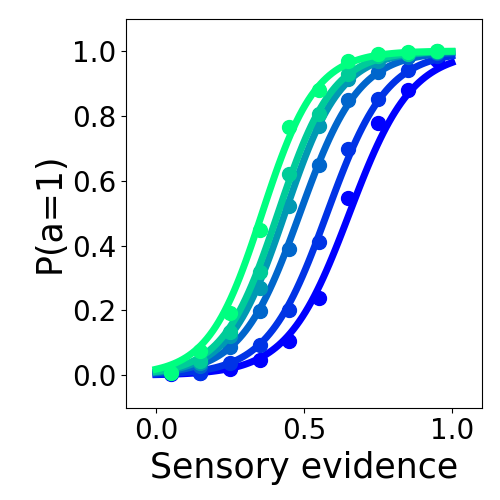
\includegraphics[width=0.5\textwidth]{images/ptask/avg_psycho_g}
  \end{figure}

\end{frame}
%%%%%%%%%%%%%%%%%%%%%%%%%%%%%%%%%%%%%%%%%%%%%%%%%%%%%%


%%%%%%%%%%%%%%%%%%%%%%%%%%%%%%%%%%%%%%%%%%%%%%%%%%%%%%
\begin{frame}{Firing rates in time}

  \begin{figure}[htb]
  \includegraphics[width=0.6\textwidth]{images/blocks}
  \end{figure}
  \vspace{-1cm}
\begin{columns}
\begin{column}{0.3\textwidth}

  \begin{figure}
  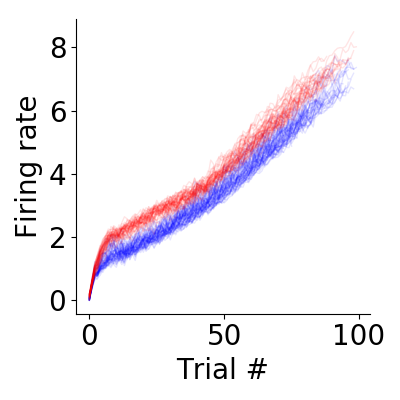
\includegraphics[width=0.9\textwidth]{images/ptask/timecourse-32}
  \end{figure}
  \vspace{-1cm}
  \begin{figure}
  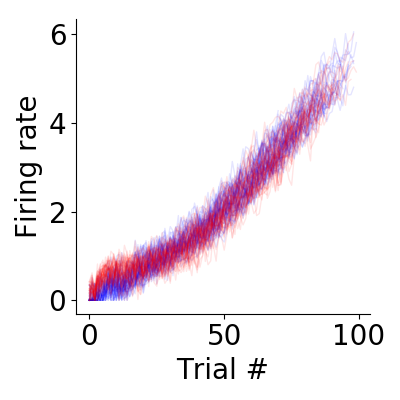
\includegraphics[width=0.9\textwidth]{images/ptask/timecourse-11}
  \end{figure}


\end{column}
\begin{column}{0.3\textwidth}

  \begin{figure}
  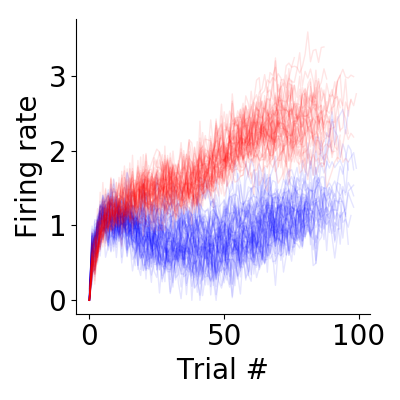
\includegraphics[width=0.9\textwidth]{images/ptask/timecourse-42}
  \end{figure}
  \vspace{-1cm}
  \begin{figure}
    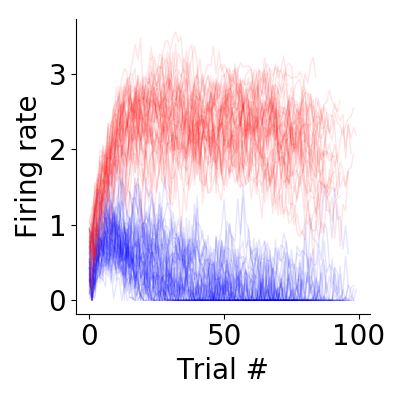
\includegraphics[width=0.9\textwidth]{images/ptask/timecourse-17}
  \end{figure}

\end{column}

\begin{column}{0.3\textwidth}

  \begin{figure}
  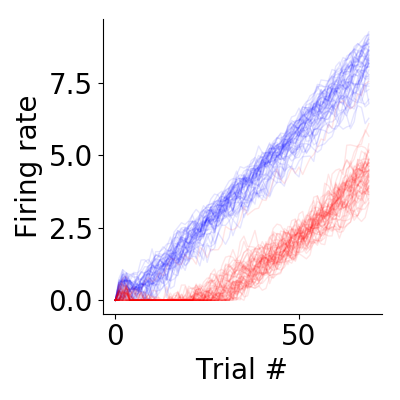
\includegraphics[width=0.9\textwidth]{images/ptask/timecourse-33}
  \end{figure}
  \vspace{-1cm}
  \begin{figure}
    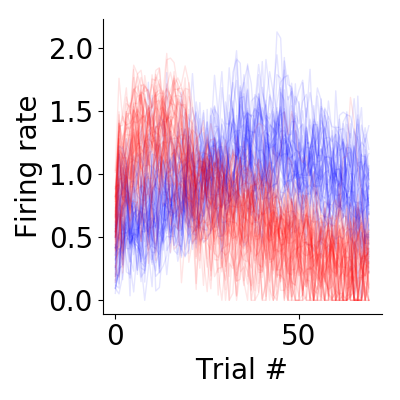
\includegraphics[width=0.9\textwidth]{images/ptask/timecourse-34}
  \end{figure}

\end{column}

\end{columns}

\end{frame}
%%%%%%%%%%%%%%%%%%%%%%%%%%%%%%%%%%%%%%%%%%%%%%%%%%%%%%

%%%%%%%%%%%%%%%%%%%%%%%%%%%%%%%%%%%%%%%%%%%%%%%%%%%%%%
\begin{frame}{Tuning curve in time}

  \begin{figure}[htb]
  \includegraphics[width=0.6\textwidth]{images/blocks}
  \end{figure}

  \begin{figure}[htb]
  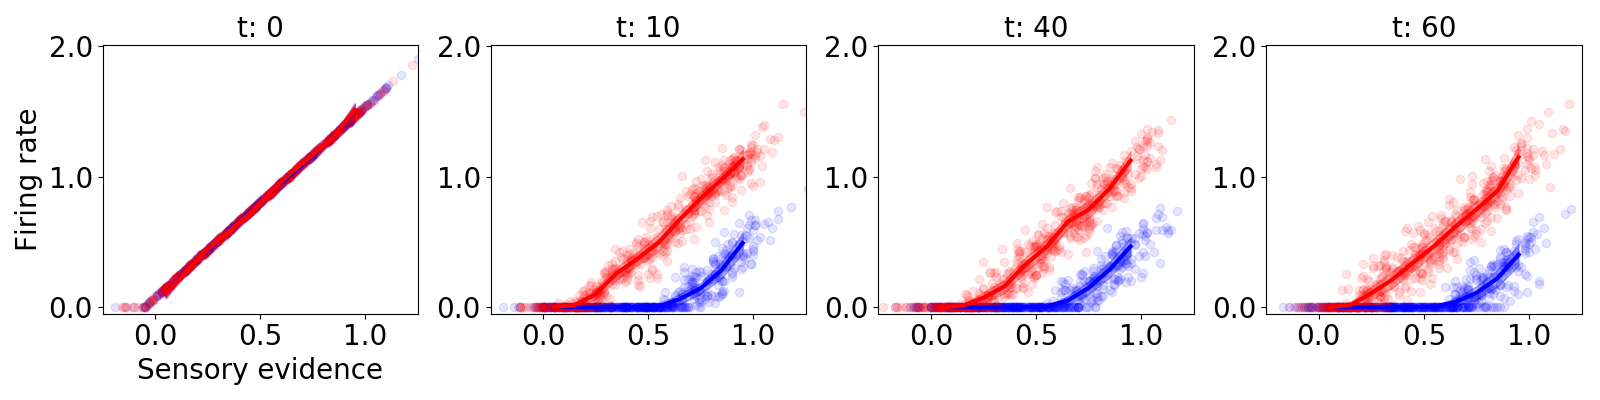
\includegraphics[width=\textwidth]{images/rtask/tuning-35}
  \end{figure}
  \vspace{-0.5cm}
  \begin{figure}[htb]
  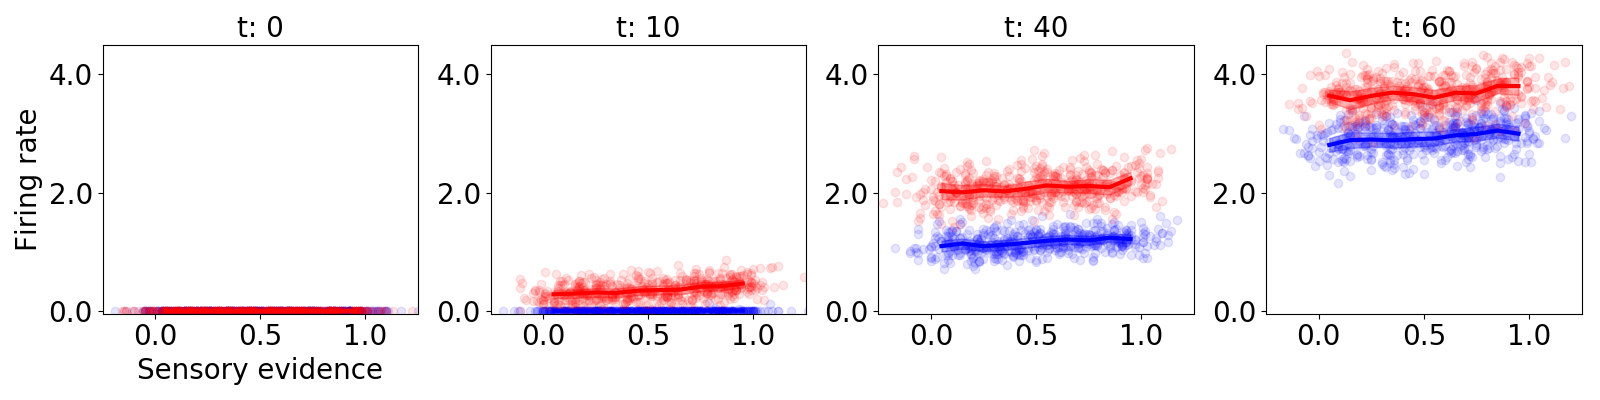
\includegraphics[width=\textwidth]{images/rtask/tuning-44}
  \end{figure}

\end{frame}
%%%%%%%%%%%%%%%%%%%%%%%%%%%%%%%%%%%%%%%%%%%%%%%%%%%%%%


%%%%%%%%%%%%%%%%%%%%%%%%%%%%%%%%%%%%%%%%%%%%%%%%%%%%%%
\begin{frame}{Discussion}

\end{frame}
%%%%%%%%%%%%%%%%%%%%%%%%%%%%%%%%%%%%%%%%%%%%%%%%%%%%%%

\begin{comment}

\begin{frame}{Open Source Fonts}
 \begin{fullpageitemize}
  \item {\montserratfont This is Montserrat}
  \item {\notosansfont This is Noto Sans}
  \item {\latolightfont This is Lato (light)}
  \item {\inconsolatafont This is inconsolata}
  \item \textsc{This is Alegreya Sans small caps}
 \end{fullpageitemize}
\end{frame}
\end{comment}

\framepic[0.8]{images/skeleton}{
 \begin{textblock}{7}(7,2.5)
    {\color{colorblue}\hugetext{\textbf{Thanks!}}}
 \end{textblock}
}

\end{document}
